
\chapter{Konzept}
\label{sec:konzept}

\section{Vorgehensweise}
\label{sec:konzept:vorgehensweise}
Für die Umsetzung in diesem Projekt eigen sich der Apriori Algorithmus (oder eine Variante davon), welcher im ersten Schritt des \nameref{sec:recherche:dataminingtechniken:disziplinen:association} (\cref{sec:recherche:dataminingtechniken:disziplinen:association}) verwendet wird sowie die \nameref{sec:recherche:dataminingtechniken:disziplinen:clusteranalysis} (\cref{sec:recherche:dataminingtechniken:disziplinen:clusteranalysis}), welche in diesem Abschnitt weiter beschrieben werden.

\nameref{sec:recherche:dataminingtechniken:disziplinen:classification} (\cref{sec:recherche:dataminingtechniken:disziplinen:classification}) fällt weg, da damit bekannte Klassen zugeteilt werden welche in diesem Projekt jedoch nicht bekannt sind. Die \nameref{sec:recherche:dataminingtechniken:disziplinen:regression} (\cref{sec:recherche:dataminingtechniken:disziplinen:regression}) eignet sich nicht, da dadurch nur numerische Werte vorausgesagt werden können, in dieser Arbeit jedoch Klassen vergeben werden müssen. \nameref{sec:recherche:dataminingtechniken:disziplinen:collaborativefiltering} (\cref{sec:recherche:dataminingtechniken:disziplinen:collaborativefiltering}) versucht durch Kundenbewertungen ähnliche Objekte vorzuschlagen. Dies kann für einen Recommender eingesetzt werden, jedoch nicht für die Auffindung von häufigen Attributen.

%Die Umsetzung in diesem Projekt wird zweistufig durchgeführt. Als erstes gibt der User eine Abfrage ein, für welche anschliessend eine eine Liste von häufig auftretenden Attributen gesucht werden soll (siehe \cref{sec:einletung:ziel} \nameref{sec:einletung:ziel}). Die Abfrage schränkt dabei den Datenbestand ein. Dafür kann der erste Schritt des \nameref{sec:recherche:dataminingtechniken:disziplinen:association} (\cref{sec:recherche:dataminingtechniken:disziplinen:association}) eingesetzt werden. Für die Analyse der Restmenge eignet sich die \nameref{sec:recherche:dataminingtechniken:disziplinen:clusteranalysis} (\cref{sec:recherche:dataminingtechniken:disziplinen:clusteranalysis}), da zu Beginn die Klassen noch nicht bekannt sind. Dadurch fällt \nameref{sec:recherche:dataminingtechniken:disziplinen:classification} (\cref{sec:recherche:dataminingtechniken:disziplinen:classification}) weg. Die \nameref{sec:recherche:dataminingtechniken:disziplinen:regression} (\cref{sec:recherche:dataminingtechniken:disziplinen:regression}) eignet sich nicht, da dadurch nur numerische Werte vorausgesagt werden können, in dieser Arbeit jedoch Klassen vergeben werden müssen. \nameref{sec:recherche:dataminingtechniken:disziplinen:collaborativefiltering} (\cref{sec:recherche:dataminingtechniken:disziplinen:collaborativefiltering}) versucht durch Kundenbewertungen ähnliche Objekte vorzuschlagen. Dies kann für einen Recommender eingesetzt werden, jedoch nicht für die Auffindung von häufigen Attributen.

% Assoziationsanalyse
%Als erstes werden Attributkombinationen (Mengen von Attributen) in der Datenbasis gesucht, welche häufig auftauchen. Dies wird durch den A-priori Algorithmus (oder Abwandlungen dadurch) erreicht. Zu Beginn wird eine mindestens Prozentzahl definiert, wie oft ein Attributmenge auftauchen muss, der sogenannte Minimal-Support. Anschliessend werden für alle 1-elementigen Mengen überpüft, ob sie den . Danach werden diese um ein Attribut erweitert und es wird erneut gezählt.  Wird dieser Wert nicht erreicht, wird die Menge als uninteressant eingestuft und nicht weiter verfolgt. 

\subsection{Einschränkung des Datenbestandes}
Im ersten Schritt wird der Datenbestand durch die Auswahl von Attributen durch den Benutzer eingeschränkt. 

%Dafür eignet sich die Häufigkeitszählung des \nameref{sec:recherche:dataminingtechniken:disziplinen:association} (\cref{sec:recherche:dataminingtechniken:disziplinen:association}), welche in diesem Abschnitt genauer beschrieben wird.

\subsection{Apriori Algorithmus}
Der Apriori Algorithmus ist der erste von zwei Schritten des \nameref{sec:recherche:dataminingtechniken:disziplinen:association} (\cref{sec:recherche:dataminingtechniken:disziplinen:association}), dessen Ziel es ist häufige Attribut-Kombinationen aufzufinden. 

Als erstes wird ein Mindestsupport $supmin$ definiert welcher Aussagt, wie oft eine Attributmenge $t$ in einer Instanz $I$ in der Datenmenge $D$ vorkommen muss, damit diese als relevant betrachtet werden kann. Der Wertebereich von $submin$ ist dabei $[0,1]$. Danach wird Iterativ die Attributmenge um ein Element erweitert und nochmals auf $submit$ überprüft. Für die Attributmenge gilt zu Beginn $|t| = k = 1$.
\begin{enumerate}
\item Für jedes $t_k$ mit $|t_k| = k$ wird gesucht wie oft es gebucht worden ist.
	\begin{center}
	$cnt(t_k) = \big|\{I \in D | t_k \subseteq I \}\big|$
	\end{center}
	Die Mengen werden in der Liste $C_k$ zusammengefasst.
\item Für jedes Attribut wird der Support $sup$ ausgerechnet.
	\begin{center}
	$sup(t_k) = \cfrac{cnt(t_k)}{|D|}$
	\end{center}
\item Es werden alle Attribute entfernt, welche $submin$ nicht erfüllen.
	\begin{center}
	$sup(t_k) \ge supmin$
	\end{center}
	Die übrig gebliebenen Mengen werden in $L_k$ vereint.
\item Es wird $L_k$ mit Elementen aus $C_k$ erweitert und ergibt $C_{k+1}$
	\begin{center}
	$ C_{k+1} = \{c \cap l | \forall c \in C_k, \forall l \in L_k \} $
	\end{center}
\item Entferne Elemente aus $C_{k+1}$, welche nicht in $L_k$ enthalten sind.
\item Wenn $C_{k+1} \neq \emptyset$ dann $k = k+1$ und gehe zu Schritt 1. 
\item Wenn $C_{k+1} = \emptyset$ dann breche ab und gib $\bigcup\limits_{i=1}^{k} L_{i}$ zurück.
\end{enumerate}

In der \cref{fig:konzept:vorgehensweise:apriorialgorithmus} wird der Ablauf noch anhand eines Beispieles veranschaulicht.

\begin{figure}[h]
	\RawFloats
	\centering
	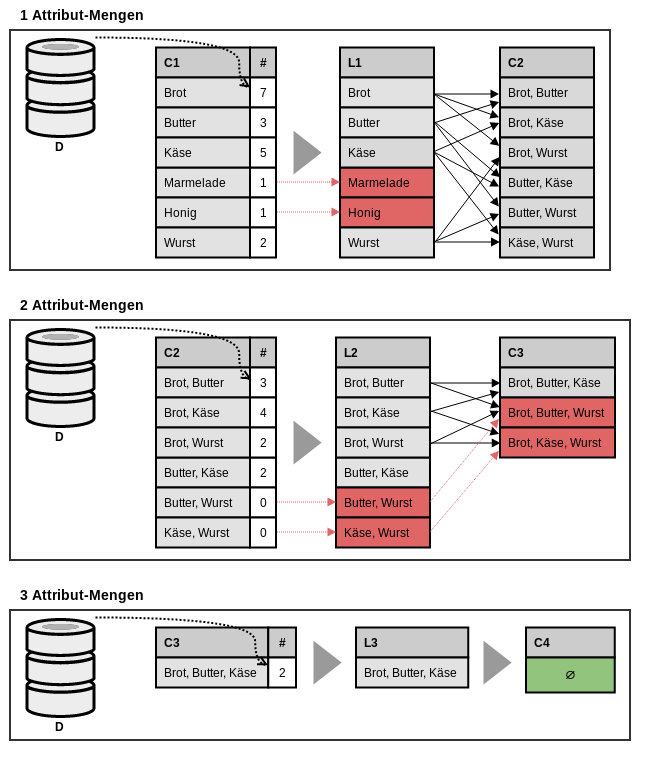
\includegraphics[width=0.8\textwidth]{images/Apriori-Algorithmus.png}
	\caption{Visualisierung des Apriori Algorithmus}
	\source{\cite{association_rule_learning_2017-01-05}}
	\label{fig:konzept:vorgehensweise:apriorialgorithmus}
\end{figure}

$D$ wird benötigt um die Vorkommen zu zählen. Die roten Elemente in $L$ werden entfernt weil $minsup$ nicht erreicht wurde, welches im Beispiel den Wert 2 hat. Die Elemente in $C$ können gelöscht werden, da sich der Apriori Algorithmus die Eigenschaft zunutze macht, dass wenn in $L_{k-1}$ ein Element $minsup$ nicht erfüllt, kann es dies auch nicht in $C_k$\todo{cite}.

Der Algorithmus kann somit in drei Schritte aufgeteilt werden.
\begin{enumerate}
\item Häufigkeitszählung
\item Generierung der x+1-Attributmenge (Apriori-gen Funktion, Join step)
\item Entfernung der Elemente welche den $minsup$ nicht erfüllen (Apriori-gen Funktion, Prune step)
\end{enumerate}

\begin{lstlisting}
procedure apriori(D: Datenmenge; minsup: Minimum support)
	$L_1$ = find_frequent_1-itemsets(D)
	for ($k = 2$; $L_{k-1} \neq \emptyset$; $k++$)
		$C_k$ = apriori_gen($L_{k-1}$)
		foreach transaction $t \in D$
			$C_t$ = subset($C_k$, $t$)
			foreach candidate $c \in C_t$
				$c$.count++;
		$L_k$ = {$c \in C_k|c$.count $\ge minsup$}
	return $\bigcup\limits_{i=1}^{k} L_{i}$
\end{lstlisting}